\relax
\tolerance10000

\item[{\bfseries(I2.1a)}]
 %{{{3
$A = -x^{-1}+C$,
\bigskip

\item[{\bfseries(I2.1b)}]
 %{{{3
$B = -t^{-1}+C$,
\bigskip

\item[{\bfseries(I2.1c)}]
 %{{{3
$C = tx^{-2}+C$,
\bigskip

\item[{\bfseries(I2.1d)}]
 %{{{3
$I = \frac12 xt^2 + C$, $J = \frac12 x^2t+C$.
\bigskip

\item[{\bfseries(I4.3)}]
 %{{{3
$ \int \sin^2x \cos^2x\, \dd
x = \frac14\int \sin^2 2x\;\dd x = \frac18\int \bigl(1-\cos 4x\bigr)\;\dd x =
\frac{x} {8} -\frac{1} {32}\sin 4x +C$.
\bigskip

\item[{\bfseries(I4.4)}]
 Rewrite the integral as %{{{3
\[
\int \cos^5\theta\;\dd \theta = \int \cos ^4\theta\,
\underbrace{\cos\theta\;\dd\theta}_{=\dd\sin\theta}
\]
and substitute $u=\sin \theta$.  We get
\begin{align*}
  \int \cos^5\theta\;\dd \theta
  &=\int \bigl(1-u^2\bigr)^2 \;\dd u\\
  &=\int \bigl(1-2u^2+u^4\bigr)\;\dd u\\
  &=u-\frac23u^3+\frac15u^5+C\\
  &=\sin\theta -\frac23\sin^3\theta + \frac15\sin^5\theta +C.
\end{align*}
For a different solution see the section on reduction formulas.
\bigskip

\item[{\bfseries(I4.5)}]
 Hopefully you remembered that $\cos^2\theta+\sin^2\theta =1$.  The %{{{3
answer is $\theta+C$.
\bigskip

\item[{\bfseries(I4.6)}]
 %{{{3
Use $2\sin A \sin B = \cos(A-B) - cos (A+B)$ to rewrite the integrand as
$\sin x\sin 2x = \frac12 \bigl(\cos (x) - \cos (3x) \bigr)$.  You then get
\[
\int \sin x\sin 2x
= \frac12 \int \bigl(\cos (x) - \cos (3x) \bigr) \; \dd x
= \frac12\sin (x) - \frac16 \sin(x) + C.
\]
\bigskip

\item[{\bfseries(I7.1)}]
 %{{{3
$\DS \int x^n \ln x\,\dd x
= \frac{x^{n+1}\ln x}{n+1} - \frac{x^{n+1}}{(n+1)^2}+C$.
\bigskip

\item[{\bfseries(I7.2)}]
 %{{{3
$\DS\int e^{ax}\sin bx\,\dd x= \frac{e^{ax}}{a^2+b^2}(a\sin bx
-b\cos bx)+C.$
\bigskip

\item[{\bfseries(I7.3)}]
 %{{{3
$\DS\int e^{ax}\cos bx\,\dd x
= \frac{e^{ax}}{a^2+b^2}(a\cos bx+b\sin bx)+C.$
\bigskip

\item[{\bfseries(I7.6)}]
 %{{{3
$\int_0^{\pi} \sin^{14}x \dd x = \frac{13\cdot11\cdot9\cdot7\cdot5\cdot3\cdot1 }
{14\cdot12\cdot10\cdot8\cdot6\cdot4\cdot2}\frac{\pi}{2}$
\bigskip

\item[{\bfseries(I7.7b)}]
 %{{{3
$\int_0^\pi \sin^5x \dd x = \frac{4\cdot2}{5\cdot3}\cdot2$\\
$\int_0^{\pi} \sin^{6}x \dd x = \frac{5\cdot3\cdot1 }
{6\cdot4\cdot2}\pi$\\
$\int_0^\pi \sin^7x \dd x = \frac{6\cdot4\cdot2}{7\cdot5\cdot3}\cdot2$
\bigskip

\item[{\bfseries(I7.8)}]
 %{{{3
$\int \cos^n x \dd x = \frac1n\sin x \cos^{n-1}x
+\frac{n-1}n\int\cos^{n-2}x \dd x$;
\[
  \int \cos^4 x\,\dd x =
  \frac38 x+ \frac14 \cos^3x\,\sin x + \frac38\cos x\,\sin x +C
\]
Setting $x=0$ and $x=\pi/4$ leads to
$\int_0^{\pi/4}\cos^4 x \dd x = \frac14+ \frac3{32}\pi$
\bigskip

\item[{\bfseries(I7.9)}]
 %{{{3
Hint: first integrate $x^m$.
\bigskip

\item[{\bfseries(I7.10)}]
 %{{{3
$x\ln x-x+C$
\bigskip

\item[{\bfseries(I7.11)}]
 %{{{3
$x(\ln x)^2-2x\ln x+2x+C$
\bigskip

\item[{\bfseries(I7.13)}]
 %{{{3
Substitute $u=\ln x$.
\bigskip

\item[{\bfseries(I7.14)}]
 %{{{3
$\int_0^{\pi/4}\tan^5 x\dd x =
\frac14(1)^4-\frac12(1)^2 + \int_0^{\pi/4}\tan x \dd x =
-\frac14+\ln\frac12\surd2$
\bigskip

\item[{\bfseries(I7.17)}]
 %{{{3
Substitute $u=1+x^2$.
\bigskip

\item[{\bfseries(I9.1a)}]
 %{{{3
$1+\frac4{x^3-4}$
\bigskip

\item[{\bfseries(I9.1b)}]
 %{{{3
$1+\frac{2x+4}{x^3-4}$
\bigskip

\item[{\bfseries(I9.1c)}]
 %{{{3
$1-\frac{x^2+x+1}{x^3-4}$
\bigskip

\item[{\bfseries(I9.1d)}]
 %{{{3
$\frac{x^3-1}{x^2-1} = x+\frac{x-1}{x^2-1}$.  You can simplify this
further: $\frac{x^3-1}{x^2-1} = x+\frac{x-1}{x^2-1} = x+\frac{1}{x+1}$.
\bigskip

\item[{\bfseries(I9.2a)}]
 %{{{3
$x^2+6x+8 = (x+3)^2-1 = (x+4)(x+2)$ so $\frac1{x^2+6x+8} =
\frac{1/2}{x+2}+\frac{-1/2}{x+4}$ and
\[
\int\frac{\dd x}{x^2+6x+8}=\frac12\ln(x+2)-\frac12\ln(x+4)+C.
\]
\bigskip

\item[{\bfseries(I9.2b)}]
 %{{{3
$\DS\int\frac{\dd x}{x^2+6x+10} = \arctan(x+3)+C.$
\bigskip

\item[{\bfseries(I9.2c)}]
 %{{{3
$\DS\frac15\int\frac{\dd x}{x^2+4x+5}= \frac15\arctan(x+2)+C$
\bigskip

\item[{\bfseries(I9.3)}]
 %{{{3
Multiply both sides of the equation
\[
\frac{x^2+3}{x(x+1)(x-1)} = \frac{A}{x}+\frac{B}{x+1}+\frac{C}{x-1}
\]
with $x(x+1)(x-1)$ and expand
\begin{align*}
  x^2+3
  &= A(x+1)(x-1)+Bx(x-1)+Cx(x+1) \\
  &= A(x^2-1)+B(x^2-x)+C(x^2+x) \\
  &=(A+B+C)x^2 +(C-B)x-A.
\end{align*}
Comparing coefficients of like powers of $x$ tells us that
\[
\left\{
\begin{aligned}
  A+B+C &=1 \\
  C-B &=0\\
  -A &= 3
\end{aligned}
\right.
\]
Therefore  $A=-3$ and $B=C=2$, i.e.
\[
\frac{x^2+3}{x(x+1)(x-1)} = -
\frac{3}{x} + \frac{2}{x+1}+\frac{2}{x-1}
\]
and hence
\[
\int \frac{x^2+3}{x(x+1)(x-1)}\,\dd x = -3\ln |x| + 2\ln |x+1|
+2\ln|x-1| + \mbox{constant}.
\]
\bigskip

\item[{\bfseries(I9.4)}]
 %{{{3
To solve
\[
\frac{x^2+3}{x(x+1)(x-1)} =
\frac{A}{x}+\frac{B}{x+1}+\frac{C}{x-1},
\]
multiply by $x$:
\[
\frac{x^2+3}{(x+1)(x-1)} = A+\frac{Bx}{x+1}+\frac{Cx}{x-1}
\]
and set $x=0$ (or rather, take the limit for $x\to0$)  to get $A=-3$; then multiply by $x+1$:
\[
\frac{x^2+3}{x(x-1)} = \frac{A(x+1)}{x}+B+\frac{C(x+1)}{x-1}
\]
and set $x=-1$
(or rather, take the limit for $x\to-1$) to get $B=2$; finally multiply by $x-1$:
\[
\frac{x^2+3}{x(x+1)} = \frac{A(x-1)}{x}+\frac{B(x-1)}{x+1}+ C,
\]
and set $x=1$ (or take the limit for $x\to-1$) to get $C=2$.
\bigskip

\item[{\bfseries(I9.5)}]
 %{{{3
Apply the method of equating coefficients to the form
\[
\frac{x^2+3}{x^2(x-1)}= \frac{A}{x}+\frac{B}{x^2}+\frac{C}{x-1}.
\]
In this problem, the Heaviside trick can still be used to find $C$
and $B$; we get $B=-3$ and $C=4$. Then
\[
\frac{A}{x}-\frac{3}{x^2}+\frac{4}{x-1}
=\frac{Ax(x-1)+3(x-1)+4x^2}{x^2(x-1)}
\]
so $A=-3$. Hence
\[
\int\frac{x^2+3}{x^2(x-1)}\,\dd x =-3\ln|x| +\frac{3}{x} +
4\ln|x-1| + \text{constant}.
\]
\bigskip

\item[{\bfseries(I9.11)}]
 %{{{3
$\frac12(x^2+\ln|x^2-1|)+C$
\bigskip

\item[{\bfseries(I9.12)}]
 %{{{3
$5\ln|x-2| -3 \ln|x-1|$.
\bigskip

\item[{\bfseries(I9.13)}]
 %{{{3
$x - 2\ln|x-1|+5\ln|x-2| + C$
\bigskip

\item[{\bfseries(I9.14)}]
 %{{{3
$\frac14\ln|e^x-1|-\frac14\ln|e^x+1|+\frac12\arctan(e^x)+C$
\bigskip

\item[{\bfseries(I9.16)}]
 %{{{3
$\arctan(e^x+1)+C$
\bigskip

\item[{\bfseries(I9.17)}]
 %{{{3
$x-\ln(1+e^x)+C$
\bigskip

\item[{\bfseries(I9.20)}]
 %{{{3
$-\ln|x|+\frac1x+\ln|x-1|+C$
\bigskip

\item[{\bfseries(I13.1)}]
 %{{{3
$\arcsin x+C$
\bigskip

\item[{\bfseries(I13.2)}]
 %{{{3
$\DS\frac12 \arcsin\frac x2 +C$
\bigskip

\item[{\bfseries(I13.3)}]
 %{{{3
$\frac12 (x\sqrt{1+{x}^{2}} + \ln|x+\sqrt{1+x^2}|\,)+C$
\bigskip

\item[{\bfseries(I13.4)}]
 %{{{3
$\arcsin(x-1)+C$
\bigskip

\item[{\bfseries(I13.13)}]
 %{{{3
$\frac13 \arctan(x+1)+C$
\bigskip

\item[{\bfseries(I13.14)}]
 %{{{3
\[
3x^2+6x+15 = 3 \bigl(x^2+2x+5\bigr) = 3\Bigl( (x+1)^2 + 4\Bigr) =
12 \Bigl(\bigl(\frac{x+1}{2}\bigr)^2 + 1\Bigr)
\]
Therefore substitute $u = \frac{x+1}{2}$.
\bigskip

\item[{\bfseries(I15.1)}]
 %{{{3
$\int_0^a x\sin x\dd x = \sin a-a\cos a$
\bigskip

\item[{\bfseries(I15.2)}]
 %{{{3
$\int_0^a x^2\cos x\dd x = (a^2+2)\sin a + 2a\cos a$
\bigskip

\item[{\bfseries(I15.3)}]
 %{{{3
$\int_3^4 \frac{x\,\dd x}{\sqrt{x^2-1}} = \left[ \sqrt{x^2-1}
\right]_3^4 =\surd15-\surd8$
\bigskip

\item[{\bfseries(I15.4)}]
 %{{{3
$\int_{1/4}^{1/3} \frac{x\,\dd x}{\sqrt{1-x^2}} = \left[ -\sqrt{1-x^2}
\right]_{1/4}^{1/3} =\frac14\surd15-\frac13\surd8$
\bigskip

\item[{\bfseries(I15.5)}]
 %{{{3
same as previous problem after substituting $x=1/t$
\bigskip

\item[{\bfseries(I15.6)}]
 %{{{3
Complete the square and substitute $u=(x+1)/4$.  See the next problem for
details.
$\frac12\ln|x^2+2x+17| - \frac14\arctan(\frac{x+1}4)+C$
\bigskip

\item[{\bfseries(I15.6)}]
 %{{{3
Completing the square leads to
\[
  \int\frac{x\,\dd x}{\sqrt{x^2+2x+17}}
  =\int \frac{x\,\dd x}{\sqrt{(x+1)^2 + 16}}
  =\frac{1}{4}\int \frac{x\,\dd x}{\sqrt{\left(\frac{x+1}{4}\right)^2 + 1}}\; .
\]
This suggests the substitution $u=\frac{x+1}{4}$, i.e.~$x=4u-1$:
\[
  \int\frac{x\,\dd x}{\sqrt{x^2+2x+17}}
  =\frac{1}{4} \int\frac{(4u-1)\cdot 4\dd u}{\sqrt{u^2+1}}
  =4\int \frac{u\,\dd u}{\sqrt{u^2+1}} - \frac{\dd u}{\sqrt{u^2+1}}.
\]
The first integral is
\[
  \int \frac{u\,\dd u}{\sqrt{u^2+1}} = \sqrt{u^2+1} (+C),
\]
which one can find by substituting $v=u^2+1$.
The second integral is in the list \ref{tbl:01inversetrig-integrals}.  Thus we
end up with
\begin{align*}
  \int\frac{x\,\dd x}{x^2+2x+17}
  &= 4\sqrt{ \Bigl(\frac{x+1}{4}\Bigr)^2+1 }
  - \ln\Bigl\{ \frac{x+1}{4} + \sqrt{ \Bigl(\frac{x+1}{4}\Bigr)^2+1 }\Bigr\} +C
  \\
  &= \sqrt{x^2+2x+17}
  - \ln\Bigl\{ \frac{x+1}{4} + \sqrt{ \Bigl(\frac{x+1}{4}\Bigr)^2+1 }\Bigr\} +C.
  \intertext{This can be further simplified to}
  &= \sqrt{x^2+2x+17}
  - \ln\Bigl\{ \frac{x+1}{4} + \frac14\sqrt{ (x+1)^2+16 }\Bigr\} +C\\
  &= \sqrt{x^2+2x+17}
  - \ln \frac{x+1 + \sqrt{ (x+1)^2+16 }}{4}  +C\\
  &= \sqrt{x^2+2x+17}
  - \ln \bigl\{ x+1 + \sqrt{ x^2+2x+17 } \bigr\} +\ln 4 +C\\
  &= \sqrt{x^2+2x+17}
  - \ln \bigl\{ x+1 + \sqrt{ x^2+2x+17 } \bigr\} +\hat C.\\
\end{align*}
\bigskip

\item[{\bfseries(I15.10)}]
 %{{{3
$\ln|x|+\frac1x+\ln|x-1|-\ln|x+1|+C$
\bigskip

\item[{\bfseries(I15.27)}]
 %{{{3
$x^2\ln(x+1) - \frac{1}{2}x^2 + x - \ln(x+1) + C$
\bigskip

\item[{\bfseries(I15.30)}]
  Substitute $x=t^2$ and integrate by parts. Answer: %{{{3
$x^2\arctan(\sqrt{x})-\sqrt{x}+\arctan(\sqrt{x})+C$
\bigskip

\item[{\bfseries(I15.33)}]
 %{{{3
$\tan(x)-\sec(x)+C$
\bigskip

\item[{\bfseries(I15.35)}]
 %{{{3
$\frac14\ln(\frac{\;(x+1)^2}{x^2+1})+\frac12\arctan(x)+C$
\bigskip

\item[{\bfseries(II4.1)}]
 %{{{3
\begin{align*}
  \int_0^\infty \frac{\dd x} {(2+x)^2}
  &= \lim_{M_\to\infty} \int_0^M \frac{\dd x} {(2+x)^2}\\
  &= \lim_{M\to\infty} \Bigl[\frac{-1} {2+x}\Bigr]_{x=0}^M \\
  &= \lim_{M|to\infty} \Bigl[\frac{-1} {2+M} - \frac{-1} {2+0}\Bigr] \\
  &= \frac{1} {2}.
\end{align*}
\bigskip

\item[{\bfseries(II4.2)}]
 %{{{3
The integrand becomes infinite as $x\to\frac{1} {2}$ so this is indeed an
improper integral.
\begin{multline*}
  \int_0^{1/2} (2x-1)^{-3}\,\dd x
  = \lim_{a\nearrow \frac12} \int_{0}^a (2x-1)^{-3} \,\dd x
  = \lim_{a\nearrow \frac12} \Bigl[-\frac14(2x-1)^{-2}\Bigr]_{0}^a\\
  = \lim_{a\nearrow \frac12} -\frac14(2a-1)^{-2} + \frac14 =-\infty.
\end{multline*}
\bigskip

\item[{\bfseries(II4.3)}]
 %{{{3
The integral is improper at $x=3$:
\[
  \int_0^{3} \frac{\dd x}{\sqrt{3-x}}
  = \lim_{a\nearrow 3} \int_0^{a} \frac{\dd x}{\sqrt{3-x}}
  = \lim_{a\nearrow 3} \Bigl[-2 \sqrt{3-x}\Bigr]_{x=0}^{x=a}
  = \lim_{a\nearrow 3} \Bigl(-2\sqrt{3-a} + 2\sqrt{3-0}\Bigr)
  = 2\surd3.
\]
\bigskip

\item[{\bfseries(II4.4)}]
 %{{{3
$2$
\bigskip

\item[{\bfseries(II4.5)}]
 %{{{3
Substitute $u=x^2$ to get the antiderivative
$\int xe^{-x^2}\,\dd x = -\frac12 e^{-x^2}+C$.  The improper integral then is:
\[
\int_0^\infty xe^{-x^2} \,\dd x =
\lim_{M\to\infty} \int_0^M xe^{-x^2} \,\dd x =
\lim_{M\to\infty} \bigl(-\frac12e^{-M^2} + \frac 12 e^{-0^2}\bigr) = \frac 12.
\]
\bigskip

\item[{\bfseries(II4.8)}]
 %{{{3
$\int_0^7x^{-1/2}\dd x = \lim_{a\searrow 0}\int_a^7 x^{-1/2}\dd x
=\lim_{a\searrow0}\bigl[2x^{1/2}\bigr]_{x=a}^7 = 2\sqrt{7}.$
\bigskip

\item[{\bfseries(II4.9)}]
 %{{{3
This integral is infinite.
\bigskip

\item[{\bfseries(II4.12)}]
 %{{{3
$\frac12 e^{-10}$
\bigskip

\item[{\bfseries(II4.13)}]
 %{{{3
$1$
\bigskip

\item[{\bfseries(II4.14)}]
 %{{{3
$\frac12$.
\bigskip

\item[{\bfseries(II4.15)}]
 %{{{3
To do the integral, substitute $x=u^2$.  The answer is $2$.
\bigskip

\item[{\bfseries(II4.21)}]
 %{{{3
$\int_1^\infty \pi r^2\, \dd x = \pi \int_1^\infty x^{-2}\dd x = \pi$
\bigskip

\item[{\bfseries(II6.3)}]
 %{{{3
$\DS\frac{x} {x^2+2x} = \frac{1} {x+2} < \frac{1} {x}$ for all $x>0$, so ``False.''
\bigskip

\item[{\bfseries(II6.4)}]
 %{{{3
True
\bigskip

\item[{\bfseries(II6.5)}]
 %{{{3
False.
\bigskip

\item[{\bfseries(II6.7)}]
 %{{{3
True because $\frac{x} {x^2+1} = \frac{1} {x+1}$.  For $x>0$ it is always true
that $x+1>x$ and therefore $\frac{1} {x} < \frac{1} {x+1}$ is true for all $x>0$.
\bigskip

\item[{\bfseries(II6.8)}]
 %{{{3
False.
\bigskip

\item[{\bfseries(II6.9)}]
 %{{{3
True.
\bigskip

\item[{\bfseries(II6.10)}]
 %{{{3
False.
\bigskip

\item[{\bfseries(II6.11)}]
 %{{{3
True.
\bigskip

\item[{\bfseries(II6.12)}]
 %{{{3
The integrand is $f(u) = \frac{u^2} {(u^2+1)^2}$, which is continuous at all
$u\geq 0$.  Therefore the integral is improper at $u\to\infty$, but nowhere else.

To determine if the integral converges we may therefore look at ``the tail,''
i.e. we can look at
\[
  I = \int_1^\infty \frac{u^2} {\bigl(u^2+1\bigr)^2} \dd u
\]
instead of the integral starting at $u=0$.

For all $u$ we have $1+u^2 \geq u^2$, and therefore
\[
  \frac{u^2}{\bigl(1+u^2\bigr)^2} \leq \frac{u^2}{(u^2)^2} = \frac{1}{u^2}.
\]
Therefore
\[
  \int_1^\infty \frac{u^2}{\bigl(1+u^2\bigr)^2} \dd u
  \leq \int_1^\infty \frac{\dd u}{u^2} = 1. \tag{\dag}
\]
This implies for the integral in the problem that
\[
  \int_0^\infty\frac{u^2}{\bigl(1+u^2\bigr)^2}\dd u <\infty.
\]
In other words the integral converges.  To get an actual estimate for how big
the integral is we already have (\dag), so we need to estimate the integral for
$0<u<1$.  On this interval we have
\[
  \frac{u^2}{\bigl(1+u^2\bigr)^2} \leq \frac{u^2}{(1)^2} = u^2,
\]
so that
\[
  \int_0^1 \frac{u^2}{\bigl(1+u^2\bigr)^2} \dd u
  \leq \int_0^1 u^2\,\dd u = \frac{1}{3}. \tag{\ddag}
\]
Therefore
\[
  \int_0^\infty \frac{u^2}{\bigl(1+u^2\bigr)^2} \dd u
  =
  \int_0^1 \frac{u^2}{\bigl(1+u^2\bigr)^2} \dd u
  +
  \int_1^\infty \frac{u^2}{\bigl(1+u^2\bigr)^2} \dd u
  \leq \frac{1}{3} + 1
  =\frac{4}{3}.
\]

\bigskip

\item[{\bfseries(II6.13)}]
 %{{{3
For large values of $u$ the integrand is approximately given by
\[
  \frac{u^3} {\bigl(u^2+1\bigr)^2} \approx \frac{u^3}{(u^2)^2} = \frac{1}{u}.
\]
Since the integral $\int_1^\infty \frac{\dd u}{u}$ diverges, we expect the
integral $I$ to diverge too.  To confirm this we try to ``estimate the tail from
below.''

For $u>1$ we have
\[
  1+u^2 < 2u^2,
\]
which implies
\[
\frac{u^3} {\bigl(u^2+1\bigr)^2} >
\frac{u^3}{(2u^2)^2} =  \frac{1}{4u}.
\]
Therefore
\[
  \int_1^\infty \frac{u^3} {\bigl(u^2+1\bigr)^2} \dd u \geq
  \int_1^\infty \frac{\dd u}{4u} =\infty.
\]
It follow that
\[
  \int_0^\infty \frac{u^3} {\bigl(u^2+1\bigr)^2}\dd u
  =
  \int_0^1\frac{u^3} {\bigl(u^2+1\bigr)^2}\dd u
  +
  \int_1^\infty\frac{u^3} {\bigl(u^2+1\bigr)^2}\dd u
  \geq
  \int_1^\infty \frac{\dd u}{4u} =\infty.
\]
In other words the integral in the problem diverges.

\bigskip

\item[{\bfseries(III4.1)}]
 %{{{3
General solution $y(x) = Ce^{\frac12 x^2}$; initial conditions imply $C=-e^{-2}$.
\bigskip

\item[{\bfseries(III4.2)}]
 %{{{3
Implicit form of the solution $\tan y = -\frac{x^2}{2}+C$, so $C=
\tan\pi/3 = \sqrt3$.

Solution $y(x) = \arctan\bigl(\sqrt3 - x^2/3\bigr)$
\bigskip

\item[{\bfseries(III4.3)}]
 %{{{3
Implicit form of the solution: $y+\frac12y^2 +x+\tfrac12x^2 =
A+\tfrac12A^2$.  If we solve for $y$ we get
\[
y = -1\pm \sqrt{A^2+2A+1-x^2-2x}
\]
Whether we need the ``$+$'' or ``$-$'' depends on $A$.
\bigskip

\item[{\bfseries(III4.4)}]
 %{{{3
Implicit form of the solution $\frac13y^3+\frac14x^4 = C$;
$C=\frac{1}{3}A^3$.  Solution is $y = \sqrt[3]{A^3-\frac34 x^4}$.
\bigskip

\item[{\bfseries(III4.5)}]
 %{{{3
Integration gives $\DS \frac12\ln\left|\frac{y-1}{y+1}\right| = x+C$.
Solve for $y$ to get $\frac{y-1}{y+1} = \pm e^{2x+2C} = \bigl(\pm
e^{2C}\bigr)e^{2x}$.

Let $B= \pm e^{2C}$ be the new constant and we get $\dfrac{y-1}{y+1} =
Be^{2x}$ whence $y = \dfrac{1+Be^{2x}}{1-Be^{2x}}$.

The initial value $y(0)=A$ tells us that $B = \frac{A-1}{A+1}$, and
therefore the solution with initial value $y(0) = A$ is $y =
\dfrac{A+1 + (A-1)e^{2x}}{A+1-(A-1)e^{2x}}$.
\bigskip

\item[{\bfseries(III4.6)}]
 %{{{3
$y(x) = \tan\bigl(\arctan (A) - x\bigr)$.
\bigskip

\item[{\bfseries(III4.7)}]
  %{{{3
$y=\sqrt{2(x-\frac{x^3}3)+1}$
\bigskip

\item[{\bfseries(III6.5)}]
  %{{{3
$y=Ce^{-2x}-\frac13 e^x$
\bigskip

\item[{\bfseries(III6.6)}]
 %{{{3
$y=xe^{\sin x}+Ae^{\sin x}$
\bigskip

\item[{\bfseries(III6.8)}]
 %{{{3
$m(x) = \cos x$, $\DS y(x) = \tan x + \frac{C} {\cos x}$, $C=0$.
\bigskip

\item[{\bfseries(III6.9)}]
 %{{{3
$\DS m(x) = \frac{1} {\cos x}$, $\DS y(x) = \tfrac12\cos x \ln\frac{1+\sin x} {1-\sin
x} + C\cos x $, $C=0$.
\bigskip

\item[{\bfseries(III6.10)}]
 %{{{3
Rewrite as $\DS  \frac{\dd y} { \dd x} +\frac{y}{\cos^2 x} =\frac {N}{\cos^2 x}$.

$m(x) = e^{\tan x}$,  $y(x) = N + C e^{-\tan x}$, $C = -N$.
\bigskip

\item[{\bfseries(III6.11)}]
 %{{{3
Rewrite as $\DS  \frac{\dd y} { \dd x} - \frac{y}{x} = 1$.

$m(x) = \frac{1} {x}$,  $y(x) = x\ln x +  C x$, $C = -\ln 2$.
\bigskip

\item[{\bfseries(III6.15)}]
 %{{{3
$y=Ce^{-x^3/3}$,\quad $C = 5e^{1/3}$
\bigskip

\item[{\bfseries(III6.16)}]
 %{{{3
$y=Ce^{-x-x^3}$,\quad $C=e^2$
\bigskip

\item[{\bfseries(III11.3a)}]
 %{{{3
Let $X(t)$ be the rabbit population size at time $t$.  The rate at which
this population grows is $dX/dt$ rabbits per year.
\begin{itemize}
\item [$\frac{5}{100}X$] from growth at 5\% per year
\item [$\frac{2}{100}X$] from death at 2\% per year
\item [$-1000$] car accidents
\item [$+700$] immigration from Sun Prairie
\end{itemize}
Together we get
\[
\frac{dX}{dt} = \frac{3}{100}X - 300.
\]
This equation is both separable and first order linear, so we can choose
from two methods to find the general solution, which is
\[
X(t) = 10,000 + C e^{0.03 t}.
\]
If $X(1991) = 12000$ then
\[
10,000 + C e^{0.03\cdot 1991} = 12,000 \implies C = 2,000e^{-0.03\cdot
1991} \text{(don't simplify yet!)}
\]
Hence
\[
X(1994) = 10,000 + 2,000e^{-0.03\cdot 1991}e^{0.03\cdot 1994} =10,000 +
2,000e^{0.03\cdot (1994-1991)} =10,000 + 2,000e^{0.09} \approx
12,188.\ldots
\]
\bigskip

\item[{\bfseries(III11.4a)}]
 %{{{3
$\sec^{-1}$.
\bigskip

\item[{\bfseries(III11.4b)}]
 %{{{3
$T_s(t) = T_r + C e^{-Kt}$.  $C$ has the same units as $T_r$ and $T_s$, so $C$ is a
temperature:  degree Fahrenheit.  $\lim_{t\to\infty} T_s(t) = T_r$: in the long run
the soup will approach room temperature.
\bigskip

\item[{\bfseries(III11.4c)}]
 %{{{3

(ii) Given $T_s(0) = 180$, $T_r=75$, and $T_s(5) = 150$. This gives the following
equations:
\[
T_r + C = 180, \quad T_r + Ce^{-5K} = 105
\implies C= 105, \quad -5K = \ln\frac{30}{105} =\ln\frac{2}{7}=-\ln\frac72.
\]
When is $T_s=90$?  Solve $T_s(t) = 90$ for $t$ using the values for $T_r$, $C$, $K$
found above ($K$ is a bit ugly so we substitute it at the end of the
problem):
\[
T_s(t) = T_r+Ce^{-Kt} = 75+105 e^{-Kt} = 90 \implies e^{-Kt} =
\frac{15}{105} = \frac{1}{7}.
\]
Hence
\[
t = \frac{\ln 1/7}{-K} = \frac{\ln 7}{K} = \frac{\ln 7}{\ln 7/2}.
\]

\bigskip

\item[{\bfseries(III11.6)}]
 %{{{3
(a) Let $y(t)$ be the amount of ``retaw'' (in gallons) in the tank at time
$t$.  Then
\[
\frac{dy}{dt} = \underbrace{\frac{5}{100}y}_{\rm growth}
- \underbrace{\quad3\quad}_{\rm removal}.
\]
(b) $y(t) = 60+ Ce^{t/20} = 60+(y_0 - 60)e^{t/20}$.

(c) If $y_0 = 100$ then $y(t) = 60 + 40 e^{t/20}$ so that
$\lim_{t\to\infty} y(t) = +\infty$.

(d) $y_0 = 60$.
\bigskip

\item[{\bfseries(III11.7)}]
 %{{{3
Finding the equation is the hard part.  Let $A(t)$ be the
\emph{volume} of acid in the vat at time $t$.  Then $A(0) = 25\%\text{ of
}1000 = 250$gallons.

$A'(t) = $ the volume of acid that gets pumped in minus the volume that gets
extracted per minute.  Per minute $40\%$ of $20$ gallons, i.e.\ 8 gallons of
acid get added.  The vat is well mixed, and $A(t)$ out of the $1000$gallons
are acid, so if 20 gallons get extracted, then $\frac{A}{1000}\cdot20$ of
those are acid.  Hence
\[
\frac{dA}{dt} = 8 - \frac{A}{1000}\cdot20 = 8-\frac{A}{50}.
\]
The solution is $A(t) = 400 + Ce^{-t/50} = 400 + (A(0)-400)e^{-t/50} = 400
-150 e^{-t/50}$.

The \emph{concentration} at time $t$ is
\[
\text{concentration} = \frac{A(t)}{\text{total volume}} =
\frac{400 - 150e^{-t/50}}{1000} = 0.4 - 0.15 r^{-t/50}.
\]
If we wait for very long the concentration becomes
\[
\text{concentration} = \lim_{t\to\infty} \frac{A(t)}{1000} = 0.4.
\]
\bigskip

\item[{\bfseries(III11.8c)}]
 %{{{3
$P$ is the volume of polluted water in the lake at time $t$.
At any time the fraction of the lake water that is polluted is $P/V$, so if
24 cubic feet are drained then $\frac{P}{V}\cdot24$ of those are polluted.
Here $V=10^9$; for simplicity we'll just write $V$ until the end of the
problem. We get
\[
\frac{dP}{dt} = \text{"in minus out"}
= 3 - \frac{P}{V} \cdot 24
\]
whose solution is $P(t) = \frac{1}{8}V+Ke^{-\frac{24}{V}t}$.  Here
$K$ is an arbitrary constant (which we can't call $C$ because in this
problem $C$ is the concentration).

The concentration at time $t$ is
\[
C(t) = \frac{P(t)}{V} = \frac18 + \frac{K}{V}e^{-\frac{24}{V}t}
=\frac18 + \bigl(C_0 - \frac18\bigr) e^{-\frac{24}{V}t} .
\]
No matter what $C_0$ is we always have
\[
\lim_{t\to\infty} C(t) = 0
\]
because $\lim_{t\to\infty} e^{-\frac{24}{V}t} = 0$.

If $C_0 = \frac18$ then the concentration of polluted water remains
constant: $C(t) = \frac18$.
\bigskip

\item[{\bfseries(IV4.1)}]
 %{{{3
Use Taylor's formula : \( Q(x)= 43+19(x-7)+\frac{11}{2}(x-7)^2 \).

A different, correct, but more laborious (clumsy) solution is to say
that $Q(x)=Ax^2+Bx+C$,, compute $Q'(x)=2Ax+B$ and $Q''(x)=2A$.  Then
\[
Q(7) = 49A + 7B + C = 43,\qquad Q'(7) = 14 A + B = 19,\qquad Q''(7) =
2A = 11.
\]
This implies $A=11/2$, $B=19-14A = 19 - 77 = -58$, and $C= 43 - 7B -
49A = 179\tfrac12$.
\bigskip

\item[{\bfseries(IV4.2)}]
 $p(x)=3+8(x-2)-\frac12 (x-2)^2$ %{{{3
\bigskip

\item[{\bfseries(IV4.17)}]
 %{{{3
$\Ti e^t = 1+ t + \frac1{2!}t^2+\cdots+\frac1{n!}t^n+\cdots$
\bigskip

\item[{\bfseries(IV4.18)}]
 %{{{3
$\Ti e^{\alpha t} = 1+\alpha t +
\frac{\alpha^2}{2!}t^2+\cdots+\frac{\alpha^n}{n!}t^n+\cdots$
\bigskip

\item[{\bfseries(IV4.19)}]
 %{{{3
$\Ti \sin(3t) = 3t-\frac{3^3}{3!}t^3 +\frac{3^5}{5!}t^5+\cdots
+\frac{(-1)^k3^{2k+1}}{(2k+1)!}t^{2k+1}+\cdots$
\bigskip

\item[{\bfseries(IV4.20)}]
 %{{{3
$\Ti \sinh t = t+\frac1{3!}t^3+\cdots+\frac1{(2k+1)!}t^{2k+1}+\cdots$
\bigskip

\item[{\bfseries(IV4.21)}]
 %{{{3
$\Ti \cosh t = 1+\frac1{2!}t^2+\cdots+\frac1{(2k)!}t^{2k}+\cdots$
\bigskip

\item[{\bfseries(IV4.22)}]
 %{{{3
$\Ti \frac1{1+2t} = 1-2t+2^2t^2-\cdots+(-1)^n2^nt^n+\cdots$
\bigskip

\item[{\bfseries(IV4.23)}]
 %{{{3
$\Ti \frac3{(2-t)^2} = \frac3{2^2} +\frac{3\cdot2}{2^3}t +
\frac{3\cdot3}{2^4}t^2+\frac{3\cdot4}{2^5}t^3
+\cdots+\frac{3\cdot(n+1)}{2^{n+2}}t^n+\cdots$ (note the cancellation
of factorials)
\bigskip

\item[{\bfseries(IV4.24)}]
 %{{{3
$\Ti \ln(1+t) =
t-\frac12t^2+\frac13t^3+\cdots+\frac{(-1)^{n+1}}{n}t^n+\cdots$
\bigskip

\item[{\bfseries(IV4.25)}]
 %{{{3
$\Ti \ln(2+2t) =\Ti \ln[ 2\cdot(1+t) ] = \ln2+\ln(1+t) = \ln2
+t-\frac12t^2+\frac13t^3+\cdots+\frac{(-1)^{n+1}}{n}t^n+\cdots $
\bigskip

\item[{\bfseries(IV4.26)}]
 %{{{3
$\Ti \ln\sqrt{1+t} = \Ti\frac12\ln(1+t) =
\frac12t-\frac14t^2+\frac16t^3+\cdots+\frac{(-1)^{n+1}}{2n}t^n+\cdots
$
\bigskip

\item[{\bfseries(IV4.27)}]
 %{{{3
$\Ti \ln(1+2t) =
2t-\frac{2^2}2t^2+\frac{2^3}3t^3+\cdots+\frac{(-1)^{n+1}2^n}{n}t^n+\cdots
$
\bigskip

\item[{\bfseries(IV4.28)}]
 %{{{3
$\Ti \ln \surd\bigl(\frac{1+t}{1-t}\bigr) = \Ti\left[
\frac12\ln(1+t)-\frac12\ln(1-t)\right] = t + \frac13t^3 +
\frac15t^5 + \cdots + \frac1{2k+1}t^{2k+1} + \cdots$
\bigskip

\item[{\bfseries(IV4.29)}]
 %{{{3
$\Ti \frac1{1-t^2} = \Ti\left[ \frac{1/2}{1-t}+\frac{1/2}{1+t}
\right]= 1+t^2+t^4+\cdots+t^{2k}+\cdots$ (we could also substitute
$x=-t^2$ in the geometric series $1/(1+x) = 1-x+x^2+\cdots$, later in
this chapter we will use ``little-oh'' to justify this point of
view.)
\bigskip

\item[{\bfseries(IV4.30)}]
 %{{{3
$\Ti \frac{t}{1-t^2} = \Ti\left[ \frac{1/2}{1-t}-\frac{1/2}{1+t}
\right] = t+t^3+t^5+\cdots+t^{2k+1}+\cdots$ (note that this function
is $t$ times the previous function so we would think its Taylor
series is just $t$ times the Taylor series of the previous function.
Again, ``little-oh'' justifies this.)
\bigskip

\item[{\bfseries(IV4.31)}]
 %{{{3
The pattern for the $n^{\text{th}}$ derivative repeats every time we
increase $n$ by 4.  So we indicate the the general terms for $n=4m,
4m+1, 4m+2$ and $4m+3$:
\[
\Ti\left( \sin t+\cos t \right)=
1+t-\frac1{2!}t^2-\frac1{3!}t^3+\frac1{4!}t^4+\cdots
+\frac{t^{4m}}{(4m)!}+\frac{t^{4m+1}}{(4m+1)!}
-\frac{t^{4m+2}}{(4m+2)!}-\frac{t^{4m+3}}{(4m+3)!}  +\cdots
\]
\bigskip

\item[{\bfseries(IV4.32)}]
 %{{{3
Use a double angle formula
\[
\Ti\left( 2\sin t\cos t \right) = \sin 2t = 2t -
\frac{2^3}{3!}t^3+\cdots+\frac{2^{4m+1}}{(4m+1)!}t^{4m+1}
-\frac{2^{4m+3}}{(4m+3)!}t^{4m+3}+\cdots
\]
\bigskip

\item[{\bfseries(IV4.33)}]
 %{{{3
$T_3\tan t = t +\frac13 t^3 $.  There is no simple general formula
for the $n^{\text{th}}$ term in the Taylor series for $\tan x$.
\bigskip

\item[{\bfseries(IV4.34)}]
 %{{{3
$\Ti \left[ 1+t^2-\frac23t^4 \right] =1+t^2-\frac23t^4$
\bigskip

\item[{\bfseries(IV4.35)}]
 %{{{3
$\Ti[(1+t)^5] = 1+5t+10t^2+10t^3+5t^4+t^5$
\bigskip

\item[{\bfseries(IV4.36)}]
 %{{{3
$\Ti\sqrt[3]{1+t} = 1 + \frac{1/3}{1!}t+\frac{(1/3)(1/3-1)}{2!}t^2
+\cdots+\frac{(1/3)(1/3-1)(1/3-2)\cdots(1/3-n+1)}{n!}t^n+\cdots$
\bigskip

\item[{\bfseries(IV4.37)}]
 %{{{3
$10! \cdot 2^6$
\bigskip

\item[{\bfseries(IV4.38)}]
 %{{{3
Because of the addition formula
\[
\sin(\alpha+\beta) = \sin\alpha\cos\beta + \sin\beta\cos\alpha
\]
we should get the same answer for $f$ and $g$, since they are the
same function!

The solution is
\begin{multline*}
  \Ti \sin(x+a) =
  \sin a + \cos(a) x - \frac{\sin a}{2!}x^2 - \frac{\cos a}{3!}x^3+\cdots \\
  \cdots + \frac{\sin a}{(4n)!}x^{4n} + \frac{\cos
  a}{(4n+1)!}x^{4n+1} - \frac{\sin a}{(4n+2)!}x^{4n+2} - \frac{\cos
  a}{(4n+3)!}x^{4n+3}+ \cdots
\end{multline*}
\bigskip

\item[{\bfseries(IV7.1)}]
 %{{{3
\[
f(x)=f^{(4)}(x)=\cos x,\qquad f^{(1)}(x)=f^{(5)}(x)= -\sin x,
\]
\[
f^{(2)}(x)=-\cos x, \qquad f^{(3)}(x)=\sin x,
\]
so
\[
f(0)=f^{(4)}(0)=1, \qquad f^{(1)}(0)=f^{(3)}(0)=0, \qquad f^{(2)}(0)=-1.
\]
and hence the fourth degree Taylor polynomial is
\[
T_4\{\cos x\}=\sum_{k=0}^4 \frac{f^{(k)}(0)}{k!}x^k
=1-\frac{x^2}{2!}+\frac{x^4}{4!}.
\]
The error is
\[
R_4\{\cos x\} = \frac{f^{(5)}(\xi)}{5!}x^5= \frac{(-\sin \xi)}{5!}x^5
\]
for some  $\xi$ between $0$ and $x$. As $|\sin \xi|\le 1$ we
have
\[
\biggl|\cos x - \left(1-\frac{x^2}{2!}+\frac{x^4}{4!}\right)\biggr|=
|R_4(x)|\le \frac{|x^5|}{5!}< \frac{1}{5!}
\]
for $|x|<1$.

Remark: Since the fourth and fifth order Taylor polynomial for
the cosine are the same, it must be that $R_4(x)=R_5(x)$.
It follows that $\frac{1}{6!}$ is also an upper bound.
\bigskip

\item[{\bfseries(IV7.3a)}]
 %{{{3
The polynomial is $p(x)=2+\frac1{12}x-\frac1{9\cdot 32}x^2$.
Then
\[
  p(1)\approx 2.07986111
\]
and the error satisfies:
\[
  |\sqrt[3]9-p(1)|\leq \frac{10}{27}\cdot8^{-\frac83}\cdot\frac1{3!}
  \approx 0.00024112654321
\]
The $\sqrt[3]{9}$ according to a computer is:
\[
  \sqrt[3]{9}\approx 2.08008382305
\]
\bigskip

\item[{\bfseries(IV9.15d)}]
 %{{{3
The PFD of $g$ is $\DS g(x) = \frac1{x-2} - \frac1{x-1}$.

$\DS g(x) = \tfrac12 + \bigl(1-\tfrac1{2^2}\bigr) x
+\bigl(1-\tfrac1{2^3}\bigr) x^2 + \cdots +
\bigl(1-\tfrac1{2^{n+1}}\bigr) x^n + \cdots$.

So $g_n = 1-1/2^{n+1}$ and $g^{(n)}(0)$ is $n!$ times that.
\bigskip

\item[{\bfseries(IV9.16)}]
 %{{{3
You could repeat the computations from problem \ref{pblm:recurrence},
and this would get us  the right answer with the same amount of work.
In this case we  could instead note that $h(x) = xg(x)$ so that
\[
h(x) = \tfrac12x + \bigl(1-\tfrac1{2^2}\bigr) x^2
+\bigl(1-\tfrac1{2^3}\bigr) x^3 + \cdots +
\bigl(1-\tfrac1{2^{n+1}}\bigr) x^{n+1} + \cdots
\]
Therefore $h_n = 1-1/2^n$.

The PFD of $k(x)$ is
\[
k(x) = \frac{2-x}{(x-2)(x-1)} \stackrel{\rm cancel!}{=} \frac1{1-x},
\]
the Taylor series of $k$ is just the Geometric series.
\bigskip

\item[{\bfseries(IV9.18)}]
 %{{{3
\(\DS\Ti e^{at} = 1 + at + \frac{a^2}{2!}t^2 + \cdots +
\frac{a^n}{n!}t^n+\cdots .\)
\bigskip

\item[{\bfseries(IV9.19)}]
 %{{{3
$e^{1+t} = e\cdot e^t$ so $\Ti e^{1+t} = e + et + \frac e{2!} t^2 +
\cdots + \frac{e}{n!}t^n + \cdots$
\bigskip

\item[{\bfseries(IV9.20)}]
 %{{{3
Substitute $u=-t^2$ in the Taylor series for $e^u$.
\[
\Ti e^{-t^2} = 1-t^2+\frac1{2!}t^4-\frac1{3!}t^6+\cdots+
\frac{(-1)^n}{n!}t^{2n} + \cdots
\]
\bigskip

\item[{\bfseries(IV9.21)}]
 %{{{3
PFD!  The PFD of $\frac{1+t}{1-t}$ is $\frac{1+t}{1-t} = -1 +
\frac2{1-t}$.  Remembering the Geometric Series we  get
\[
\Ti \frac{1+t}{1-t} = 1 + 2t + 2t^2+2t^3+\cdots +2t^n+\cdots
\]
\bigskip

\item[{\bfseries(IV9.22)}]
 %{{{3
Substitute $u=-2t$ in the Geometric Series $1/(1-u)$.  You get
\[
\Ti \frac1{1+2t} = 1-2t+2^2t^2-2^3t^3 + \cdots + \cdots + (-1)^n2^n t^n
+\cdots
\]
\bigskip

\item[{\bfseries(IV9.23)}]
 $f(x)=1-\frac{x^2}{3!}+ \frac{x^4}{5!}-\cdots$ %{{{3
$=\sum_{n=0}^\infty \frac{(-1)^n}{(2n+1)!}\;{x^{2n}}$
\bigskip

\item[{\bfseries(IV9.24)}]
 %{{{3
\begin{multline*}
  \Ti\frac{\ln (1+x)}{x} =
  \frac{x-\frac12x^2+\frac13x^3+\cdots+(-1)^{n-1}\frac1nx^n+\cdots}{x}\\
  = 1-\frac12 x +\frac13 x^2 + \cdots + (-1)^{n-1}\frac1nx^{n-1}+\cdots
\end{multline*}
\bigskip

\item[{\bfseries(IV9.25)}]
 %{{{3
\[
\Ti \frac{e^t}{1-t} = 1 + 2t + \bigl(1+1+\tfrac1{2!}\bigr)t^2
+\bigl(1+1+\tfrac1{2!}+\tfrac1{3!}\bigr)t^3 +
\cdots+\bigl(1+1+\tfrac1{2!}+\cdots +\tfrac1{n!}\bigr)t^n+\cdots
\]
\bigskip

\item[{\bfseries(IV9.26)}]
 %{{{3
$1/\sqrt{1-t} = (1-t)^{-1/2}$ so
\[
\Ti\frac1{\sqrt{1-t}} = 1 +\tfrac12 t + \frac{\tfrac12 \tfrac32}{1\cdot
2} t^2 +\frac{\tfrac12 \tfrac32 \tfrac52}{1\cdot 2\cdot 3}t^3+\cdots
\]
(be careful with minus signs when you compute the derivatives of
$(1-t)^{-1/2}$.)

You can make this look nicer if you multiply top and bottom in the
$n^{\rm th}$ term with $2^n$:
\[
\Ti\frac1{\sqrt{1-t}} = 1 + \frac12 t + \frac{1\cdot3}{2\cdot 4}t^2
+\frac{1\cdot3\cdot5}{2\cdot4\cdot6}t^3+\cdots
+\frac{1\cdot3\cdots(2n-1)}{2\cdot4\cdots2n}t^n+\cdots
\]
\bigskip

\item[{\bfseries(IV9.27)}]
 %{{{3
\[
\Ti\frac1{\sqrt{1-t^2}} = 1 + \frac12 t^2 + \frac{1\cdot3}{2\cdot 4}t^4
+\frac{1\cdot3\cdot5}{2\cdot4\cdot6}t^6+\cdots
+\frac{1\cdot3\cdots(2n-1)}{2\cdot4\cdots2n}t^{2n}+\cdots
\]
\bigskip

\item[{\bfseries(IV9.28)}]
 %{{{3
\[
\Ti\arcsin t = t + \frac12 \frac{t^3}{3} + \frac{1\cdot3}{2\cdot 4}
\frac{t^5}{5} +\frac{1\cdot3\cdot5}{2\cdot4\cdot6}\frac{t^7}{7}+\cdots
+\frac{1\cdot3\cdots(2n-1)}{2\cdot4\cdots2n}\frac{t^{2n+1}}{2n+1}+\cdots
\]
\bigskip

\item[{\bfseries(IV9.29)}]
 %{{{3
$T_4 [e^{-t}\cos t] = 1-t+\frac13 t^3 - \frac16 t^4$.
\bigskip

\item[{\bfseries(IV9.30)}]
 %{{{3
\(\displaystyle T_4 [e^{-t}\sin 2t] = t-t^2+\frac13t^3+o(t^4)\) (the
$t^4$ terms cancel).
\bigskip

\item[{\bfseries(IV9.31)}]
 %{{{3
PFD of $1/(2-t-t^2) = \frac1{(2+t)(1-t)} = \frac{-\frac13}{2+t} +
\frac{\frac13}{1-t}$.  Use the geometric series.
\bigskip

\item[{\bfseries(IV9.32)}]
 %{{{3
$\sqrt[3]{1+2t+t^2} = \sqrt[3]{(1+t)^2} = (1+t)^{2/3}$.  This is very
similar to problem \ref{pblm:for-the-arcsine}.  The answer follows from
Newton's binomial formula.
\bigskip

\item[{\bfseries(IV11.1b)}]
 The Taylor series is %{{{3
\[
\sin(t)=t-t^3/6+\cdots
\]
and  the order one and two Taylor polynomial is
the same $p(t)=t$.
For any $t$ there is a $\zeta$ between
$0$ and $t$ with
$$\sin(t)-p(t)=\frac{f^{(3)}(\zeta)}{3!}t^3$$
When $f(t)=\sin(t)$,
$|f^{(n)}(\zeta)|\leq 1$
for any $n$ and $\zeta$.
Consequently, $$|\sin(t)-p(t)|\leq \frac{t^3}{3!}$$
for nonnegative $t$.
Hence
$$|\int_0^{\frac12} \sin(x^2)\;dx - \int_0^{\frac12} p(x^2)\;dx|\leq
\int_0^{\frac12} |\sin(x^2)-p(x^2)|\;dx \leq
\int_0^{\frac12} \frac{x^6}{3!} \; dx =
\frac{(\frac12)^7}{3!\; 7}=\epsilon $$
Since $\int_0^{\frac12} p(x^2)\;dx = \frac{\;(\frac12)^3}{3}=A$
(the approximate value)
we have that
$$ A-\epsilon\leq  \int_0^{\frac12} \sin(x^2)\;dx
\leq A+\epsilon$$
\bigskip

\item[{\bfseries(IV11.2c)}]
 (b) $\frac{43}{30}$ (c) $\frac{3}{6!\cdot 13}$  %{{{3
\bigskip

\item[{\bfseries(V3.1)}]
 %{{{3
$1/2$
\bigskip

\item[{\bfseries(V3.2)}]
 %{{{3
Does not exist (or ``$+\infty$'')
\bigskip

\item[{\bfseries(V3.3)}]
 %{{{3
$1/2$
\bigskip

\item[{\bfseries(V3.4)}]
 %{{{3
$-1$
\bigskip

\item[{\bfseries(V3.5)}]
 %{{{3
$0$
\bigskip

\item[{\bfseries(V3.6)}]
 %{{{3
Does not exist (or ``$-\infty$'') because $e>2$.
\bigskip

\item[{\bfseries(V3.7)}]
 %{{{3
$0$.
\bigskip

\item[{\bfseries(V3.8)}]
 %{{{3
$0$.
\bigskip

\item[{\bfseries(V3.9)}]
 %{{{3
$0$ (write the limit as $ \limntoi \frac{n!+1}{(n+1)!} =\limntoi
\frac{n!}{(n+1)!} + \limntoi \frac{1}{(n+1)!} = \limntoi \frac{1}{n+1}
+ \limntoi \frac{1}{(n+1)!}$).
\bigskip

\item[{\bfseries(V3.11)}]
 %{{{3
Use the explicit formula (\ref{eq:fibonacci-explicit}) from Example
\ref{ex:fibonacci-2}.  The answer is the Golden Ratio $\phi$.
\bigskip

\item[{\bfseries(V6.1)}]
 The remainder term $R_n(x)$ is equal to %{{{3
$\frac {f^{(n)}(\zeta_n)}{n!}x^n$ for some $\zeta_n$.
For either the cosine or sine and any $n$ and $\zeta$
we have $|{f^{(n)}(\zeta)}|\leq 1$.  So
$|R_n(x)|\leq \frac{\;|x|^n}{n!}$. But we know
$\lim_{n\to\infty} \frac{|x|^n}{n!} =0$ and hence
$\lim_{n\to\infty} R_n(x) =0$.
\bigskip

\item[{\bfseries(V6.2)}]
\def\soc{\mathrm{soc}}% %{{{3
The $k^{\rm th}$ derivative of $g(x) = \sin(2x)$ is $g^{(k)}(x) = \pm
2^k \soc(2x)$.  Here $\soc(\theta)$ is either $\sin \theta$ or $\cos
\theta$, depending on $k$.  Therefore $k^{\rm th}$ remainder term is
bounded by
\[
|R_k[\sin 2x]| \leq \frac{|g^{(k+1)}(c)|} {(k+1)!}|x|^{k+1} =\frac
{2^{k+1}|x|^{k+1}}{(k+1)!} |\soc (2x)| \leq \frac{|2x|^{k+1}} {(k+1)!}.
\]
Since $\lim_{k\toi} \frac{|2x|^{k+1}} {(k+1)!} = 0$ we can use the
Sandwich Theorem and conclude that $\lim_{k\toi}R_k[g(x)] = 0$, so the
Taylor series of $g$ converges for every $x$.
\bigskip

\item[{\bfseries(V6.6)}]
 %{{{3
Read the example in \S\ref{ex:nochemistry}.
\bigskip

\item[{\bfseries(V6.7)}]
 %{{{3
$-1 < x <1$.
\bigskip

\item[{\bfseries(V6.8)}]
 %{{{3
$-1<x<1$.
\bigskip

\item[{\bfseries(V6.9)}]
 %{{{3
$-1 < x < 1$.
\bigskip

\item[{\bfseries(V6.10)}]
 %{{{3
$-\frac 32 < x < \frac 32$.  Write $f(x)$ as $f(x) = \frac 13 \frac
1{1-(-\frac23x)}$ and use the Geometric Series.
\bigskip

\item[{\bfseries(V6.11)}]
 $|x|<2/5$  %{{{3
\bigskip

\item[{\bfseries(VI9.3e)}]

(a) $3$ \quad
(b) $\tvek 2 \\ -4 \\ 4 \ttor$  \quad
(c) 36  \quad
(d) $\tvek 3 \\ -3 \\ 3 \ttor$  \quad
(e) $\tvek 1 \\ -5 \\ 5 \ttor$
\bigskip

\item[{\bfseries(VI9.6c)}]

(a) Since $\vek 1 \\ 2 \tor +\vek x \\ x \tor = \vek 1+x \\ 2+x\tor$ the number
$x$ would have to satisfy both $1+x=2$ and $2+x=1$.  That's impossible, so
there is no such $x$.

(b) No drawing, but $\vp = \vek 1 \\ 2 \tor +\vek x \\ x \tor =
\vek 1\\ 2\tor + x \vek 1\\ 1\tor$ is the parametric representation of a
straight line through the points $(1,2)$ (when $x=0$) and $(2,3)$ (when
$x=1$).

(c) $x$ and $y $ must satisfy $\vek x+y \\ 2x+y\tor = \vek 2\\ 1\tor$.  Solve
$x+y = 2$, $2x+y = 1$ to get $x=-1$, $y=3$.
\bigskip

\item[{\bfseries(VI9.7)}]

Every vector is a position vector.  To see of which point it is the position
vector translate it so its initial point is the origin.

Here $\tpv AB = \vek -3\\ 3 \tor$, so $\tpv AB$ is the position vector of
the point $(-3,3)$.
\bigskip

\item[{\bfseries(VI9.8)}]

One always labels the vertices of a parallelogram counterclockwise (see
\S\ref{sec:diag-parall}).

$ABCD$ is a parallelogram if $\tpv AB + \tpv AD = \tpv AC$.
$\tpv AB = \vek 1\\ 1 \tor$, $\tpv AC = \vek 2\\ 3 \tor$, $\tpv AD = \vek 3\\
1 \tor$.  So $\tpv AB + \tpv AD \ne \tpv AC$, and $ABCD$ is not a
parallelogram.
\bigskip

\item[{\bfseries(VI9.9a)}]

As in the previous problem, we want $\tpv AB + \tpv AD = \tpv AC$.
If $D$ is the point $(d_1, d_2, d_3)$ then
$\tpv AB = \vek 0\\ 1\\1 \tor$,
$\tpv AD = \vek d_1\\ d_2-2 \\ d_3-1\tor$,
$\tpv AC = \vek 4\\ -1\\ 3 \tor$,
so that $\tpv AB + \tpv AD = \tpv AC$ will hold if
$d_1 = 4$, $d_2 = 0$ and $d_3 = 3$.
\bigskip

\item[{\bfseries(VI9.9b)}]

Now we want $\tpv AB + \tpv AC = \tpv AD$, so $d_1 = 4$, $d_2 = 2$,
$d_3 = 5$.
\bigskip

\item[{\bfseries(VI10.3b)}]

(a)
$\vx = \vek 3\\ 0\\1 \tor + t \vek -1\\ 1\\1 \tor = \vek 3-t\\ t\\ 1+t \tor$.

(b) Intersection with $xy$ plane when $z=0$, i.e.\ when $t=-1$, at $(4, -1,
0)$.
Intersection with $xz$ plane when $y=0$, when $t=0$, at $(3,0,1)$ (i.e.\ at
$A$).  Intersection with $yz$ plane when $x=0$, when $t=3$, at $(0, 3, 4)$.
\bigskip

\item[{\bfseries(VI10.4b)}]

(a) $\vec{L}[t]=\tvek 2 \\ 3 \\ 1 \ttor+t\tvek 1 \\ -1 \\ 2 \ttor$
\par (b) $\tvek 4 \\ 1 \\ 5 \ttor$
\bigskip

\item[{\bfseries(VI10.5c)}]

(a) $\vp = (\vb+\vc)/2$,  $\vq = (\va+\vc)/2$, $\vr = (\va+\vb)/2$.

(b) $\vm = \va + \frac23(\vp-\va)$  (See Figure \ref{fig:line-through-AB},
with $AX$ twice as long as $XB$).  Simplify to get
$\vm = \frac13\va + \frac13\vb + \frac13\vc$.

(c) Hint : find the point $N$ on the line segment $BQ$ which is twice as far
from $B$ as it is from $Q$.  If you compute this carefully you will find that
$M=N$.
\bigskip

\item[{\bfseries(VI11.1)}]

To decompose $\vb$ set $\vb= \vb_\perp+\vb_\pll$, with $\vb_\pll = t\va$ for
some number $t$.  Take the dot product with $\va$ on both sides and you get
$\va\dpp\vb = t\|\va\|^2$, whence $3 = 14 t$ and $t=\frac3{14}$.  Therefore
\[
  \vb_\pll = \frac{3}{14}\va, \qquad \vb_\perp = \vb-\frac{3}{14}\va.
\]
To find $\vb_\pll$ and $\vb-\perp$ you now substitute the given values for
$\va$ and $\vb$.


The same procedure leads to $\va_\perp$ and $\va_\pll$:
$\va_\pll = \frac{3}{2}\vb$, $\va_\perp = \va - \frac32\vb$.
\bigskip

\item[{\bfseries(VI11.2)}]

This problem is of the same type as the previous one, namely we have to
decompose one vector as the sum of a vector perpendicular and a vector
parallel to the hill's surface.  The only difference is that we are not given
the normal to the hill so we have to find it ourselves.  The equation of the
hill is $12x_1 + 5x_2 = 130$ so the vector $\vn = \tvek 12\\ 5\ttor$ is a
normal.

The problem now asks us to write $\vf_{\rm grav} = \vf_\perp + \vf_\pll$,
where $\vf_\perp = t\vn$ is perpendicular to the surface of the hill, and
$\vf_\pll$ id parallel to the surface.

Take the dot product with $\vn$, and you find $t\|\vn\|^2 =
\vn\dpp\vf_{\rm grav} \implies 169t = -5mg \implies t=-\frac{5}{169}mg$.
Therefore
\[
  \vf_\perp = -\frac{5}{169}mg\vek12 \\5\tor
  =\vek -\frac{60}{169}mg \\ -\frac{25}{169}mg\tor,
  \qquad
  \vf_\pll = \vf_{\rm grav} - \vf_\perp
  = \vek -\frac{60}{169}mg \\ \frac{144}{169}mg\tor,
\]
\bigskip

\item[{\bfseries(VI12.1c)}]

$\|\va-\vb\|^2 = \|\va\|^2 - 2\va\dpp\vb + \|\vb\|^2$;
$\|2\va-\vb\|^2 = 4\|\va\|^2 - 4\va\dpp\vb + \|\vb\|^2$;
$\nm{\va+\vb} = \sqrt{54}$, $\nm{\va-\vb} = \sqrt{62}$ and
$\nm{2\va-\vb}=\sqrt{130}$.
\bigskip

\item[{\bfseries(VI12.3)}]

Compute $\tpv AB = -\tpv BA = \vek 1\\ 1\tor$,
$\tpv BC = -\tpv CB = \vek -2 \\ 2 \tor$,
$\tpv AC = -\tpv CA = \vek -1 \\ 3 \tor$.
Hence
$\|\tpv AB\| = \sqrt{2}$,
$\|\tpv BC\| = \sqrt{8} = 2\sqrt{2}$,
$\|\tpv AC\| = \sqrt{10}$.

And also $\tpv AB\dpp \tpv AC = 2 \implies \cos \angle A =
\frac{\tpv AB\dpp \tpv AC}{\|\tpv AB\|\,\|\tpv AC\|} =
\frac{2}{\sqrt{20}} = \frac{1}{\sqrt{5}}$.

A similar calculation gives $\cos \angle B = 0$ so we have a right triangle;
and $\cos\angle C = \frac{2}{\sqrt{5}}$.
\bigskip

\item[{\bfseries(VI12.4)}]

$\tpv AB = \tvek2\\1\ttor$,
$\tpv AC = \tvek t-1\\ 2-t\ttor$,
$\tpv BC = \tvek t-3 \\1-t\ttor$.

If the right angle is at $A$ then $\tpv AB \dpp \tpv AC = 0$, so that
we must solve $2(t-1) + (2-t) = 0$. Solution: $t=0$, and $C = (0,3)$.

If the right angle is at $B$ then $\tpv AB \dpp \tpv BC = 0$, so that
we must solve $2(t-3) + (1-t) = 0$. Solution: $t=5$, and $C = (5, -2)$.

If the right angle is at $C$ then $\tpv AC \dpp \tpv BC = 0$, so that
we must solve $(t-1)(t-3) + (2-t)(1-t) = 0$. Note that this case is
different in that we get a quadratic equation, and in that there are two
solutions, $t=1$, $t=\frac52$.

This is a complete solution of the problem, but it turns out that there is a
nice picture of the solution, and that the four different points $C$ we find
are connected with the circle whose diameter is the line segment $AB$:
\begin{center}
  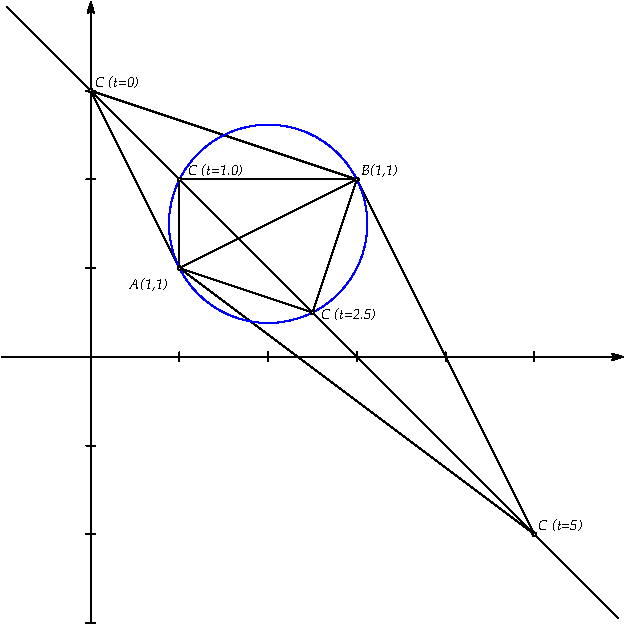
\includegraphics{05rightangle-problem.pdf}
\end{center}
\bigskip

\item[{\bfseries(VI12.5a)}]

$\ell$ has defining equation $-\frac12 x + y = 1$ which is of the form
$\vn\dpp\vx = $constant if you choose $\vn = \tvek-1/2 \\ 1\ttor$.
\bigskip

\item[{\bfseries(VI12.5b)}]

The distance to the point $D$ with position vector $\vd$ from the line
$\ell$ is $\frac{\vn\dpp(\vd-\va)}{\|\vn\|}$ where $\va$ is the position
vector of any point on the line.  In our case $\vd = \vvv0$
and the point $A(0,1)$, $\va = \tpv OA = \tvek 0\\1\ttor$, is on the line.
So the distance to the origin from the line is $\dfrac{-\vn\dpp\va}{\|\vn\|}
= \dfrac{1}{\sqrt{(1/2)^2 + 1^2}} = 2/\sqrt{5}$.
\bigskip

\item[{\bfseries(VI12.5c)}]

$3x+y=2$, normal vector is $\vm = \tvek3\\1\ttor$.
\bigskip

\item[{\bfseries(VI12.5d)}]

Angle between $\ell$ and $m$ is the angle $\theta$ between their normals,
whose cosine is $\cos \theta = \frac{\vn\dpp\vm}{\|\vn\|\,\|\vm\|} =
\frac{-1/2}{\sqrt{5/4}\sqrt{10}} = -\frac{1}{\sqrt{50} }=
-\frac{1}{10}\sqrt{2}$.
\bigskip

\item[{\bfseries(VI13.3a)}]

$\vvv0$ (the cross product of any vector with itself is the zero vector).
\bigskip

\item[{\bfseries(VI13.3c)}]

$(\va+\vb)\cp (\va-\vb) = \va\cp\va +\vb\cp\va - \va\cp\vb - \vb\cp\vb =
-2\va\cp\vb$.
\bigskip

\item[{\bfseries(VI13.4)}]

Not true.  For instance, the vector $\vc$ could be $\vc = \va+\vb$, and
$\va\cp\vb$ would be the same as $\vc\cp\vb$.
\bigskip

\item[{\bfseries(VI13.5a)}]

A possible normal vector is $\vn = \tpv AB \cp \tpv AC = \tvek-4\\4\\-4\ttor$.
Any (non zero) multiple of this vector is also a valid normal.  The nicest would
be $\frac14\vn = \tvek-1\\1\\-1\ttor$.
\bigskip

\item[{\bfseries(VI13.5b)}]

$\vn\dpp(\vx-\va) = 0$, or $\vn\dpp\vx = \vn\dpp\va$.  Using $\vn$ and
$\va$ from the first part we get $-4x_1 + 4x_2 -4x_3 = -8$.  Here you could
replace $\va$ by either $\vb$ or $\vc$. (Make sure you understand why; if you
don't think about it, then ask someone).
\bigskip

\item[{\bfseries(VI13.5c)}]

Distance from $D$ to $\cP$ is $\frac{\vn\dpp(\vd-\va)}{\|\vn\|} =
4/\sqrt{3} = \frac43\sqrt{3}$.  There are many valid choices of normal
$\vn$ in part (i) of this problem, but they all give the same answer here.

Distance from $O$ to $\cP$ is $\frac{\vn\dpp(\vvv0-\va)}{\|\vn\|} =
\frac23\sqrt{3}$.
\bigskip

\item[{\bfseries(VI13.5d)}]

Since $\vn\dpp(\vvv0-\va)$ and $\vn\dpp(\vd-\va)$ have the same sign the point
$D$ and the origin lie on the same side of the plane $\cP$.
\bigskip

\item[{\bfseries(VI13.5e)}]

The area of the triangle is $\frac12\|\tpv AB\cp\tpv AC\| = 2\sqrt{3}$.
\bigskip

\item[{\bfseries(VI13.5f)}]

Intersection with $x$ axis is $A$, the intersection with $y$-axis occurs at
$(0,-2,0)$ and the intersection with the $z$-axis is $B$.
\bigskip

\item[{\bfseries(VI13.6a)}]

Since $\vn = \tpv AB\cp\tpv AC = \tvek-3\\1\\1\ttor$ the plane through
$A,B,C$ has defining equation $-3x+y+z = 3$.  The coordinates $(2,1,3)$ of
$D$ do not satisfy this equation, so $D$ is not on the plane $ABC$.
\bigskip

\item[{\bfseries(VI13.6b)}]

If $E$ is on the plane through $A,B,C$ then the coordinates of $E$ satisfy the
defining equation of this plane, so that $-3\cdot1+1\cdot1+1\cdot\alpha = 3$.
This implies $\alpha=5$.
\bigskip

\item[{\bfseries(VI13.7a)}]

If $ABCD$ is a parallelogram then the vertices of the parallelogram are labeled
$A$, $B$, $C$, $D$ as you go around the parallelogram in a counterclockwise
fashion. See the figure in \S43.2.

Then $\tpv AB + \tpv AD = \tpv AC$.  Starting from this equation there
are now two ways to solve this problem.

\textbf{(first solution)}  If $D$ is the point $(d_1, d_2, d_3)$ then $\tpv AD =
\tvek d_1-1 \\d_2+1\\d_3-1\ttor$, while $\tpv AB = \tvek1\\1\\0\ttor$ and $\tpv
AC = \tvek0\\3\\-1\ttor$. Hence $\tpv AB + \tpv AD = \tpv AC$ implies
$\tvek d_1 \\d_2+2 \\d_3-1\ttor = \tvek0\\3\\-1\ttor$, and thus
$d_1 = 0$, $d_2 = 1$ and $d_3 = 0$.

\textbf{(second solution)} Let $\va, \vb, \vc, \vd$ be the position vectors of $A,B,C,D$.
Then $\tpv AB = \vb-\va$, etc.\ and $\tpv AB + \tpv AD = \tpv AC$ is equivalent
to $\vb-\va + \vd-\va = \vc-\va$.  Since we know $\va, \vb, \vc$ we can solve
for $\vd$ and we get
$\vd = \vc-\vb+\va = \tvek1\\-1\\1\ttor - \tvek2\\0\\1\ttor + \tvek1\\2\\0\ttor
= \tvek0\\1\\0\ttor$.
\bigskip

\item[{\bfseries(VI13.7b)}]

The area of the parallelogram $ABCD$ is $\|\tpv AB \cp \tpv AD\| =
\left\|\tvek-1\\1\\3\ttor\right\| = \sqrt{11}$.
\bigskip

\item[{\bfseries(VI13.7c)}]

In the previous part we computed $\tpv AB \cp \tpv AD = \tvek-1\\1\\3\ttor$, so
this is a normal to the plane containing $A,B,D$.  The defining equation for
that plane is $-x+y+3z = 1$.  Since $ABCD$ is a parallelogram any plane
containing $ABD$ automatically contains $C$.
\bigskip

\item[{\bfseries(VI13.7d)}]

$(-1,0,0)$, $(0,1,0)$, $(0,0,\frac{1}{3})$.
\bigskip

\item[{\bfseries(VI13.8a)}]
 Here is the picture of the parallelepiped (which you can also find on
page 103):
\begin{center}
  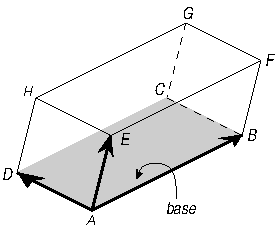
\includegraphics{05parallelepiped2.pdf}
\end{center}
Knowing the points $A, B, D$ we get $\tpv AB = \tvek-1\\2\\0\ttor$,
$\tpv AD = \tvek-2\\0\\1\ttor$.  Also, since $\parppd EFGHABCD$ is a
parallelepiped, we know that all its faces are parallelogram, and thus $\tpv EF
= \tpv AB$, etc.  Hence: we find these coordinates for the points $A$,
$B$, \dots

$A(1,0,0)$, (given);
$B(0,2,0)$, (given);
$C(-2,2,1)$, since $\tpv AC = \tpv AB + \tpv AD = \tvek-3\\2\\1\ttor$;
$D(-1,0,1)$, (given);
$E(0,0,2)$, (given)\\
$F(-1,2,2)$, since we know $E$ and  $\tpv EF = \tpv AB = \tvek -1\\2\\0\ttor$\\
$G(-3,2,3)$, since we know $F$ and  $\tpv FG =\tpv EH = \tpv AD = \tvek -2\\0\\1\ttor$\\
$H(-2,0,3)$, since we know $E$ and  $\tpv EH = \tpv AD = \tvek -2\\0\\1\ttor$.
\bigskip

\item[{\bfseries(VI13.8b)}]

The area of $ABCD$ is $\| \tpv AB\cp\tpv AD\| = \sqrt{21}$.
\bigskip

\item[{\bfseries(VI13.8c)}]

The volume of $\mathfrak P$ is the product of its height and the area of its
base, which we compute in the previous and next problems.  So
height$=\frac{\rm volume}{\rm area\, base} = \frac{6}{\sqrt{21}} =
\frac{2}{7}\sqrt{21}$.
\bigskip

\item[{\bfseries(VI13.8d)}]

The volume of the parallelepiped is $\tpv AE\dpp(\tpv AB \cp \tpv AD) = 6$.
\bigskip
